\documentclass{sig-alternate}

\usepackage{url}
\usepackage{graphicx}
\usepackage{caption}
\usepackage{subcaption}
\usepackage{hyperref}
\usepackage{url}
\usepackage{times}
\usepackage{balance}
\usepackage{xspace}
\usepackage{paralist}
\usepackage{color}

\clubpenalty = 10000
\widowpenalty = 10000
\displaywidowpenalty = 10000

\begin{document}

\newcommand{\ghtorrent}{\textsc{ght}orrent\xspace}
\newcommand{\prioritizer}{\textsc{pr}ioritizer\xspace}
\newcommand{\api}{\textsc{api}\xspace}
\newcommand{\todo}[1]{\textcolor{red}{\textbf{\textsc{todo:}} #1}}

\newcommand{\nb}[3]{
  \fcolorbox{black}{#2}{\bfseries\sffamily\scriptsize#1}
    {\sf\small$\blacktriangleright$\textit{#3}$\blacktriangleleft$}
}

\newcommand\georgios[1]{\nb{Georgios}{yellow}{#1}}
\newcommand\andy[1]{\nb{Andy}{cyan}{#1}}
\newcommand\erik[1]{\nb{Erik}{magenta}{#1}}

\newcommand{\hassanbox}[1]
{
  \vspace{0.29em}
  \noindent
  \fbox{
  \begin{minipage}{0.46\textwidth}
    \emph{\noindent #1}
    \end{minipage}
}}

% Macros for qualitative research :-)
\newcommand{\resp}[2]{{\sc R#1:} ``\emph{#2}''}
\newcommand{\respnum}[1]{{\sc R#1}}
\newcommand{\code}[1]{{\textsl{#1}}}

\title{Prioritizer paper}

\author{
\alignauthor
Erik van der Veen\\
       \affaddr{Delft University of Technology}\\
       \affaddr{Delft, the Netherlands}\\
       \email{e.v.d.veen@tudelft.nl}
\and
Georgios Gousios\\
       \affaddr{Radboud Universiteit Nijmegen}\\
       \affaddr{Nijmegen, the Netherlands}\\
       \email{georgios@cs.ru.nl}
\and
Andy Zaidman\\
       \affaddr{Delft University of Technology}\\
       \affaddr{Delft, the Netherlands}\\
       \email{a.zaidman@tudelft.nl}
}

\maketitle

\begin{abstract}

\end{abstract}

\category{D.2.7}{Software Engineering}{Distribution, Maintenance, and Enhancement}[Version control]
\category{D.2.9}{Software Engineering}{Management}[Programming teams]

\terms{Management}

\keywords{pull-based development, pull request, distributed software development,
empirical software engineering}

\section{Introduction}

\section{Background and Related Work}

\section{Research Questions}

\section{Study Design}
\label{sec:design}


\section{Implementation}
\label{sec:implementation}

To test whether it is possible to prioritize PRs we have designed a service that automatically tries to do just that.

\subsection{Features}
\label{sec:features}

For creating system that automatically creates an ordered list of PRs, we tried to use a machine algorithm that ranks the incoming PRs according a set of features.
Most of the features we use are based on features that are used by many integrators to manually sort their PRs \cite{GZSD15}.

\begin{description}
\item[Age]
The number of minutes between the moment the PR was opened to the current time.
There is a large group of integrators that take a PR's age into account when manually prioritizing their PRs.

\item[Target Branch]
The name of the branch the PR is targeting in the base repository.
It makes sense to use the target branch not as string, but as a categorical variable.
Unfortunately the ML algorithm chokes if there is a new branch value that was not part of the training data.
Therefore this feature is not included in the training data at all, but it is still available for manual sorting (see visualizer in \ref{sec:architecture}).

\item[Core Member]
A boolean value indicating whether the author of the pull request is a core member of the project.
Some integrators value PRs of members more than those of non-members.

\item[Intra-Branch]
A boolean value indicating whether the pull request is coming from another branch of the same base project.
Creating these kind of PRs requires write access to the repository, so they can only be created by core members.

\item[Contains Fix]
A boolean value indicating whether the pull request contains some sort of bug fix rather than e.g. a feature.
This is really just an indication as the value is only true if the PR contains the string ``fix'' in its title.
In general PRs with a fix are prioritized over other PRs.

\item[Contribution Rate]
The number of commits that is already included in the project \emph{and} authored by the pull requester divided by the total number of commits in the project.
I.e. the contribution rate of the PR author.
There are integrators that look at PRs of known contributers first, their code is of known quality and often faster to review.
On the other hand there are also integrators that value PRs of new contributors more than those of known contributers.
The rationale behind this is that new contributers are feeling more valued when they receive a fast response on their PR.
Possibly will that feeling encourage them to continue to contribute the to project.

\item[Accept rate]
The number of accepted (i.e. merged) pull requests authored by the current pull requester divided by the total number of PRs he/she authored.
I.e. the accept rate of the PR author.
A high accept rate can indicate that the author already gained some trust by the integrator, which can result in a higher prioritity.
This feature suffers possibly from accuracy problems, as it is difficult to determine whether a PR is actually merged or not.
A pull request can be merged in different ways \cite{GPD14}.
A merge performed via the GitHub interface is easy to detect, but a PR which is squashed to one commit before the merge is difficult to detect.

\item[Comments]
There are different types of comments that can be made regarding a pull request.
This feature counts the number of comments on the issue that is automatically created along the pull request.
Usually a general dicussion about the PR takes place within the issue.
The number of comments might indicate whether a PR needs more/less attention.

\item[Review Comments]
Review comments are comments on a portion of the unified diff of a pull request.
These are separate from issue comments, which do not reference a portion of the unified diff.
This feature counts the number of review comments on a PR.

\item[Last Comment Mention]
A boolean value indicating whether the last comment on a request (regardless of the comment type) contains a mention to a GitHub user.
A comment with a mention contains ``@username'' anywhere in the body of the comment.
The mention suggests that the user who is mentioned needs to take action.

\item[Additions]
The number of lines added by the pull request.
Together with the following three features it captures the size of a PR.
A very large group uses the size of the change to manually prioritize their PRs.

\item[Deletions]
The number of lines deleted by the pull request.

\item[Commits]
The number of commits contained by the pull request.

\item[Files]
The number of files changed by the pull request.

\item[Has Test Code]
A boolean value indicating whether the pull request contains changes to test files.
Some projects have a extensive test suite.
In these projects it is often expected that new PRs contain tests for the code they add.
The heuristic used for the test code detection is simple, the value of the feature is true if the PR changes at least one file with ``test'' or ``spec'' in its file name.

\item[Pairwise conflicts]
When the conflicts among different PRs are known it can be used to determine a merge order in which the number of conflicts is reduced.
Pairwise conflicts are only checked among PRs which target the same branch
\end{description}

\subsection{Architecture}
\label{sec:architecture}

Our implementation of the service consists of several components.
Figure \ref{fig:architecture} shows a global overview of the architecture.
The \prioritizer service uses two main data sources: GitHub and the \ghtorrent project.
The latter provides a message queue which can be used to subscribe to pull request events.
When such an event arrives the \emph{watcher} component of the \prioritizer is notified (1) and starts prioritizing the project (2).
When the \emph{analyzer} gets a prioritization request it fetches the list of PRs from GitHub (3).
At the same time it fetches the pull request contents to the local Git clone.
When the data is fetched the analyzer starts enriching the PR list with data from the local clone and \ghtorrent (4).
This step calculates and adds several of the features to the PRs.
The data is now ready to be processed by the \emph{predictor} (5) which gives a certain rank to the PRs.
After the ordered list is returned to the analyzer (6), the output is generated and available for the \emph{visualizer} (7).
Details about the different components are discussed in the following sections.

\begin{figure}
  \centering
  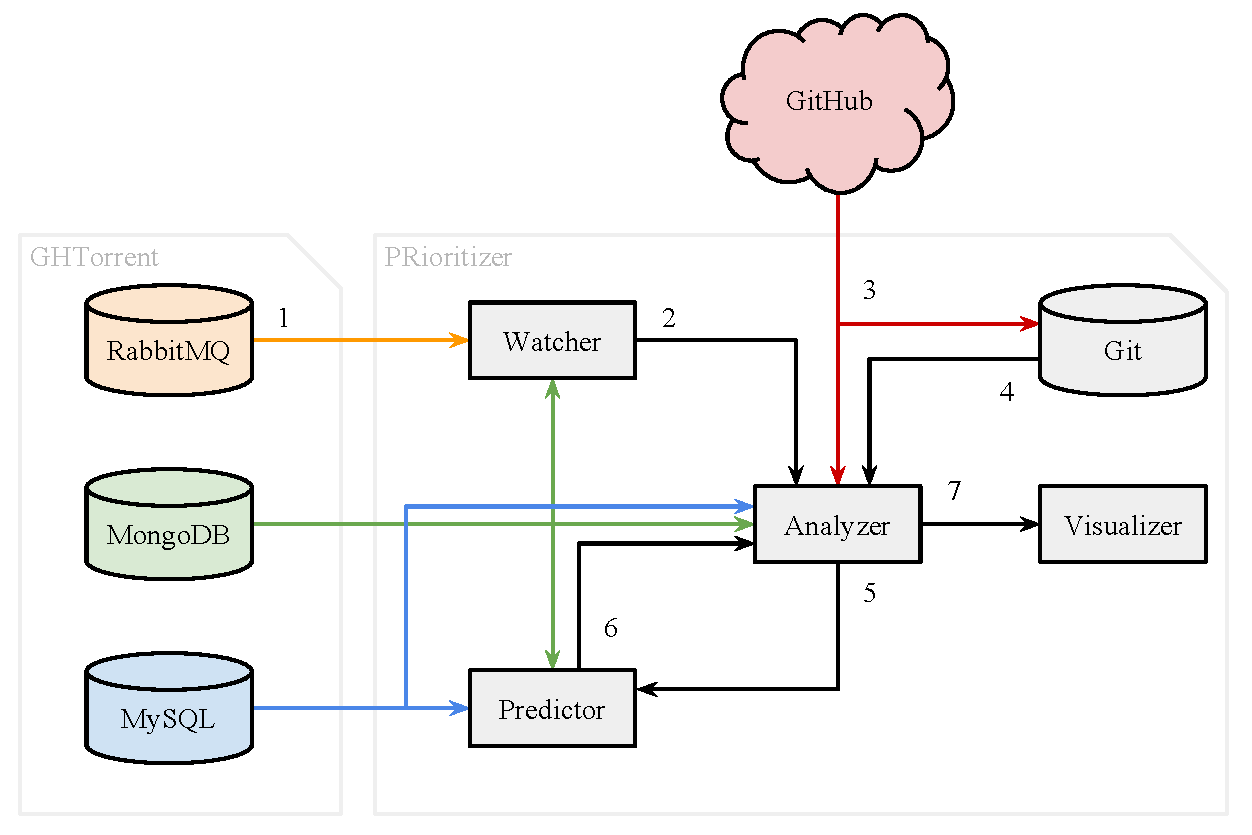
\includegraphics[width=0.5\textwidth]{../figs/architecture.pdf}
  \caption[Diagram of the architecture]
   {Diagram of the architecture. It shows the different data sources and components used by the \prioritizer service.}
  \label{fig:architecture}
\end{figure}

\begin{description}
\item[Watcher]
At the beginning of the chain we have the watcher, it is implemented in the Scala programming language.
The watcher continuously listens to pull request event from \ghtorrent via a RabbitMQ message queue.
Pull request events are triggered when a PR is assigned, unassigned, labeled, unlabeled, opened, closed, reopened, or synchronized.
The PR events of all public repositories on GitHub are received by the watcher.
Incoming events from repositories that are not currently tracked are discarded by the watcher.
If an event is received from a tracked repository the analyzer is invoked for that specific repository.

\item[Analyzer]
The component at the center of the service is the analyzer, it is also implemented in Scala.
When the analyzer kicks in, it receives a repository name from the watcher.
An up-to-date list of open PRs for that repository is fetched from GitHub through the GitHub \api.
In parallel the local git clone is updated with commits of the latest PRs.
At the time both processes are finished, the list with PRs is enriched with data from \ghtorrent as well as the local git clone.

The enrichment process adds e.g. information about the pull request author like the \emph{accept rate}, the \emph{contributor rate} and others described in section \ref{sec:features}.
To retrieve information like the mergability and the \emph{pairwise conflicts} of the PRs the local git clone is used.
Pairwise conflicts are only checked among PRs which target the same branch, but nevertheless the amount of pairs can be very high.
In the worst case, i.e. when all PRs target the same branch, the number of pairs to be checked is $O(n^2)$.
Therefore this is the most time consuming feature of the service.
After the enrichment process is done, the list is written to a repository specific cache.
This enables a faster enriching process in future runs, especially the pairwise conflict check benefits from the cache.

Some of the enrichment information (e.g. the mergability or number of comments) is also available directly via the GitHub \api.
However, this data is only present when requesting a single PR, whereas a request for a list of 100 PRs lacks this sort of data.
This means that if we want this data directly from GitHub we have to create one \api request per pull request.
When prioritizing PRs for a large amount of repositories it consumes also a large amount of \api requests and reaches GitHub's maximum of 5,000 requests/hour quickly.
So, our solution to this problem is to use \ghtorrent instead.

Before the final output is written to the disk, the predictor is invoked on the enriched PR list.
A list of ordered PRs is returned back from the predictor to the analyzer.
Details about this process are in the next paragraph.
The analyzer completes its process with writing the ordered list of PRs to the disk in JSON format, which will be picked up by the visualizer.

\item[Predictor]
The predictor assigns a rank to every pull request, it is partly written in Scala and partly in R.
When the predictor receiver a list of PRs it first checks if there is already a up-to-date prediction model.
If this is not the case, the first step is to train the prediction model on a set of PRs from the past.

The training process consists of two phases, first the historical data must be retrieved and secondly the actual model must be trained.
Information about closed pull request, their comments and their authors is harvested from \ghtorrent.
Once all data is fetched, the lifetime of each PR is divided into time windows as explained in section \ref{sec:ml}.
Then for each time window the state of a pull request, its comments and its author is determined.
If a certain time window contains an event or action, then the previous window is marked as \emph{important}.
All other windows are marked as \emph{not important}.
Each of these time windows (with its state) is a row in the training data.
When the training set is complete it is passed to the R program which trains the prediction model.

The Random Forest machine learning algorithm, called in R, learns what features are important for dividing the PRs in two classifications (important vs. not important).
The resulting model is saved to the disk for later use when predicting the ranks.

Once we have a up-to-date prediction model, we can use it for ordering the PR list.
The list and the model are feeded to the prediction algorithm in R.
Using the prediction model each PR is given a probability that it belongs to the \emph{important} cluster.
A PR with a high probability means that it is more likely to receive an event or action (from the user) soon.
We interpret PRs with a high probability as PRs that need attention, therefore the ranked list of PRs is obtained by ordering the list on the importance probability from high to low.
The final list is then returned to the analyzer.

\item[Visualizer]
The visualizer is a user interface for the ordered list, it is a web application written in HTML and Javascript.
An example view of the interface can be seen in figure \ref{fig:ui}.
To make the development faster and easier we used AngularJS, a Javascript framework.
The visualizer is a static website which accesses the JSON produced by the analyzer.
When a specific repository is requested by the user, the corresponsding JSON file is parsed and showed on the web page.

The list is automatically sorted on the rank outputted by the predictor.
However, the user is also able to sort or filter manually on different fields and features.
On GitHub has only a limited set of fields available to sort and filter on.
The visualizer interface provides more sort and filter options based on the features from section \ref{sec:features} e.g. conflicts, author properties or size.
Sorting on something trivial as the size of a PR is not support on GitHub while many integrators use it as manual prioritization feature \cite{GZSD15}.

The interface tells users on which PR they have to focus first.
However, to actually take action the user still has to go to GitHub's interface.
To make it easier for the user each PR in the list has a link to the GitHub version.
Futhermore, if a user wants more information about a specific PR, he/she can click the PR to reveal more details about the features.
\end{description}

\begin{figure}
  \centering
  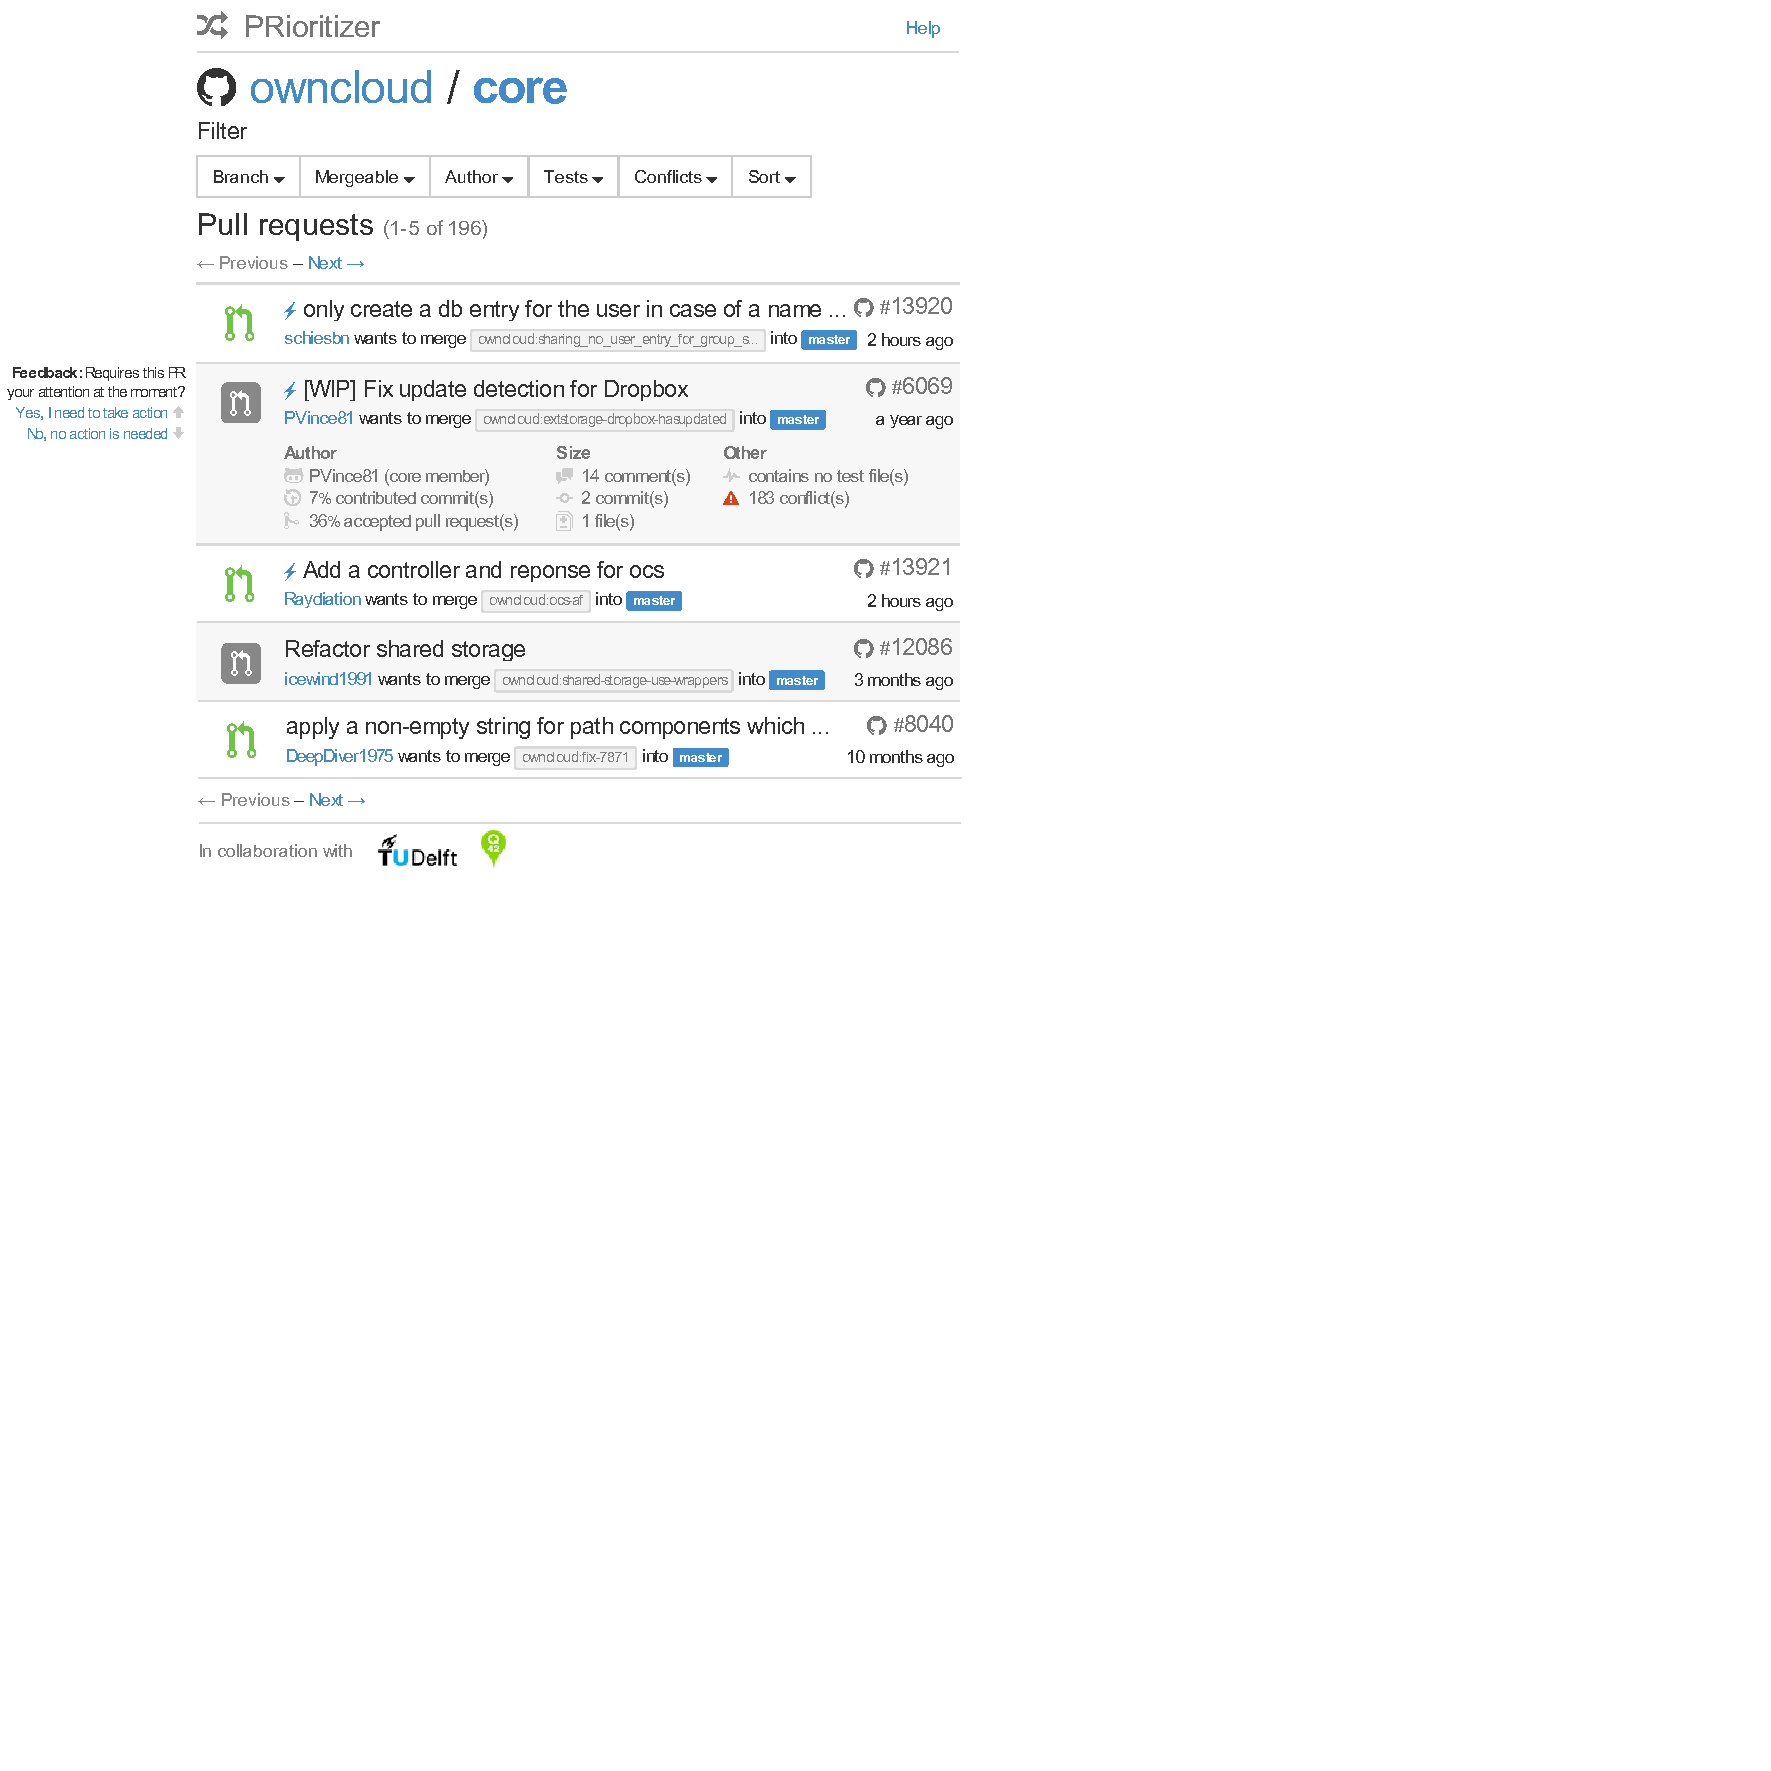
\includegraphics[width=0.5\textwidth]{../figs/interface.pdf}
  \caption[The user interface]
   {The user interface. It shows an ordered list of pull requests that need attention.}
  \label{fig:ui}
\end{figure}


\section{Experimental Setup}

\section{Results}

\section{Discussion}

\section{Limitations}

\section{Conclusions}

\bibliographystyle{IEEEtran}
\bibliography{prioritizer}


\end{document}
